\chapter{Программная реализация модуля}

\section{Выбор технических средств решения задачи}

Как показали результаты обзора существующих тестовых фреймворков, на данный момент нет решения польностью
удовлетворяющего поставленным требованиям. Однако многие рассмотренные программные комплексы уже предоставляют часть
необходимого нам функционала, поэтому для решения поставленной на дипломный
проект задачи нет необходимсти создавать тестовую утилиту с нуля, разумнее
будет выбрать одно из существующих решений, и доработать его.
Чтобы выбрать из предложенного разнообразия подходящий продукт, составим таблицу, где укажем, в какой степени каждый
тестовый фреймворк удовлетворяет поставленным требованиям.

ТУТ ТАБЛИЦА

Анализ показал, что оптимальным выбором, в наибольшей степени удовлетворяющим поставленным требованиям, является
Apache JMeter. Именно на базе его функционала будет реализовано решение задачи дипломногот проекта.

Разработка модуля будет осуществляться с использованием языка Java, что обусловлено одним из требований технического
задания --- кросплатформенность приложения. Программы на Java транслируются в байт-код, выполняемый виртуальной машиной
Java (JVM) --- программой, обрабатывающей байтовый код и передающей инструкции оборудованию как интерпретатор, что
обеспечивает полную независимости байт-кода от операционной системы и оборудования и позволяет выполнять
Java-приложения на любом устройстве, для которого существует соответствующая виртуальная машина. Также выбранный нами
тестовый фреймворк Apache JMeter является стопроцентным Java приложением, поэтому для интеграции с ним целесообразно
использовать именно этот язык.

На текущий момент основным средством обеспечения взаимодействия Flex клиентов с Java приложениями является технология
BlazeDS --- серверная Java-технология для передачи данных, поддерживающая AMF протокол. BlazeDS является бесплатным
приложением с открытым исходным кодом,разработано компанией Adobe. В силу распространённости BlazeDS, одно из основных
функциональных требований к реализации модуля --- обработка AMF сообщений --- будет решаться с помощью средств именно
этой техноогии.

В качестве инструмента автоматизации сборки проектов был выбран Apache Maven  фреймворк для автоматизации сборки
проектов, специфицированных на XML-языке POM (Project Object Model).Основными преимуществами Maven являются:

\begin{enumerate}
\item Независимость от OS. Сборка проекта происходит в любой операционной системе. Файл проекта один и тот же.
\item Управление зависимостями. Редко какие проекты пишутся без использования сторонних библиотек(зависимостей), которые
 зачастую тоже в свою очередь используют библиотеки разных версий. Мавен позволяет управлять такими сложными
 зависимостями, что позволяет разрешать конфликты версий и в случае необходимости легко переходить на новые версии
 библиотек.
\item Возможна сборка из командной строки. Такое часто необходимо для автоматической сборки проекта на сервере
(Continuous Integration).
\item Хорошая интеграция с средами разработки. Основные среды разработки на java легко открывают проекты которые
собираются c помощью maven. При этом зачастую проект настраивать не нужно --- он сразу готов к дальнейшей разработке.
Как следствие - если с проектом работают в разных средах разработки, то maven удобный способ хранения настроек.
Настроечный файл среды разработки и для сборки один и тот же --- меньше дублирования данных и соответственно ошибок.
\item Декларативное описание проекта. B файлах проекта pom.xml содержится его декларативное описание, а не отдельные
команды.
\end{enumerate}

Эффективность разработки программного обеспечения в любом современном проекте подразумевает возможность вести
разработку параллельно с другими участниками проекта.Для оптимизации совместной работы над дипломным проектом было
принято решение о размещении всех файлов проекта в репозитории системы контроля версий Git. Git --- это быстрая,
масштабируемая, распределенная система управления версиями с большим набором команд, которые обеспечивают как
операции верхнего уровня, так и полный доступ к внутренним механизмам.

В качестве среды разработки бал выбрана IntellijIdea\cite{idea-book}.

\section{Реализация поддержки AMF протокола}

\subsection{Общие сведения о BlazeDS}
BlazeDS --- серверная Java-технология для передачи данных. Предоставляет ряд сервисов, которые позволяют приложениям
клиента взаимодействовать с сервером, а также осуществяет передачу данных между несколькими клиентами, подключенными 
к серверу BlazeDS, в режиме реального времени.BlazeDS приложение состоит из двух частей: клиентского приложения и серверного 
J2EE web-приложения. Данная архитектура представлена на следующем рисунке

ТУТ РИСУНОК

Клиентское приложение BlazeDS обычно представляет собой Adobe Flex или AIR приложение. В его состав входят: 

\begin{enumerate}
\item Пользовательский интерфейс приложения. Создаётся с помощью Flex SDK;
\item Один или несколько компонентов BlazeDS: 
\begin{enumerate}
\item RemoteObject --- компонент, предоставляющий клиентскому приложению доступ к методам Java-объектов на стороне сервера; 
\item HTTPService --- компонент, позволяющий клиентскому приложению с помощью http запросов взаимодействовать с JSP, сервлетами, 
ASP страницами через сервер BlazeDS;
\item WebService --- компонент, предназанченный для взаимодействия с веб-сервисами;
\item Producer --- компонент-отправитель сообщений, предназанчен для взаимодействия с сервером сообщений;
\item Consumer --- компонент-получатель сообщений, предназанчен для взаимодействия с сервером сообщений.
\end{enumerate}
\item Набор каналов. На стороне клиента определяются каналы,которые инкапсулируют соединение между Flex клиентом и сервером 
BlazeDS. Для клиентского приложения задаётся набор каналов, упорядоченных по предпочтению. Flex компонент пытается подключиться 
по первому каналу, указанному в списке, и в случае неудачи выбирает следующий канал и т.д, до тех пор пока соединение не будет 
установлено, либо список каналов не кончится.Flex клиенты могут использовать различные типы каналов, такие как AMFChannel и 
HTTPChannel. AMFChannel использует бинарный AMF протокол, а HTTPChannel - небинарный формат AMFX (AMF, преобразованный в XML). 
Выбор канала зависит от ряда факторов, например от типа создаваемого приложения, формата передачи данных, требуемого размера 
сообщений.
\end{enumerate}

Архитектура сервера BlazeDS представлена на ...

Тут РИСУНОК

BlazeDS сервер базируется на технологии J2EE. Взаимодействие клиента и сервера BlazeDS происхоит следующим 
образом : Flex клиент посылает запрос по определённому каналу, далее запрос направляется в соответствующий каналу 
компонент endpoint, который является точкой обработки получаемых сервеом сообщений различного типа. Затем сообщение 
декодируется и проходит через ряд Java-объектов - MessageBroker , Service object, Destination object и Adapter object.
Adapter object либо обрабатывает запрос локально, либо связывается с какой-либо backend системой или
удалённым сервером. После запроса происходит обратный процесс.
 
Таким образом для обеспечения поддержки AMF протокола в разрабатываемом программном 
обеспечении, необходимо будет реализовать модуль, осуществляющий сериализацию сообщений 
перед их отправкой от клиента к серверу и наоборот, десериализацию полученных клиентом сообщений 
сервера.

\subsection{Сериализация и десериализация сообщений}

Рассмотрим подробнее спецификацию AMF.

AMF --- бинарный формат, используемый для сериализации структурированных данных, таких как объекты Action Script или
XML, и обмена сообщениями между Adobe Flash клиентом и удалённым сервисом. Action Message Format более экономичен 
по трафику по сравнению с XML и позволяет передавать типизированные объекты. Первая версия протокола, AMF0, была 
применена в Flash Player 6 в 2001 и оставалась неизменной в реализациях ActionScript 2.0 в Flash Player 7 и Flash 
Player 8. В Flash Player 9 был внедрён Action Script 3.0 с усовершенствованной виртуальной машиной 
ActionScript Virtual Machine (AVM+). В новой версии протокола, AMF3, оптимизирован формат сообщений и введена 
поддержка новых типов. Далее будет рассматриваться именно обновлённая версия протокола.

AMF протокол поддерживает следующие типы данных:

\begin{enumerate}
\item undefined --- любой неcпецифицированный протоколом формат данных;
\item null;
\item boolean;
\item integer --- в ActionScript 3.0 integer представляет собой 29х битное число переменной длины без знака или 28 битное
со знаком. Если выделенных битов не достаточно для представления числа, то AVM+ сериализует его как тип double;
\item double --- 8ми байтовое число с плавающей точкой в формате IEEE 754 с порядком байтов от старшегок младшему
(network byte order)
\item string --- сторка в кодировке UTF-8, литерал или ссылка;
\item xml-doc --- данные в xml формате в кодировке UTF-8. При сериализации преобразуются в строку;
\item date --- сериализуется как число миллисекунд, прошедших с 00:00:00 первого января 1970 в часовом поясе UTC,
данные о локальном часовом поясе не посылаются;
\item array --- массивы данных;
\item object --- amf3 обрабатывает Action Script объекты, а также разработанные пользователем классы, которые можно
разделить на следующие группы:
\begin{enumerate}
\item анонимные --- Action Script объекты или экземпляры пользовательских классов, не имеющие зарегистрированных в
протоколе псевдонимов. В процессе десериализации анонимные объекты будут интерпретироваться как Object;
\item типизированные --- экземпляры классов с зарегистрированными в протоколе псевдонимами;
\item динамические --- экземпляры классов, общедоступные переменные которых могут динамически изменяться во время
выполнения кода;
\item сериализуемые --- экземпяры классов, реализующих интерфейс flash.utils.IExternalizable, которые полностью
контролируют сериализацию своих членов.
\end{enumerate}
\item xml --- в Action Script 3.0 введена поддержка XML синтаксиса E4X;
\item byte-array --- в Action Script 3.0 введён новый формат хранения массива байтов, ByteArray. AMF3 сериализует
данные этого типа с использованием 29ти битного значения, передаваемого в качестве длины массива байтов.
\end{enumerate} 

AMF сообщение содержит информацию об отдельной транзакции. Оно определяют вызываемую удалённую операцию, 
операцию, выполняемую клиентом в случае успеха или ошибки запроса, и используемые при этом данные. Структуры сообщений,
представляющих запросы клиента и ответы сервера, одинаковы.
 
Первым полем AMF сообщения является target URI, которое описывает, какая операция, функция или 
метод должны быть вызваны. Спецификация AMF не определяет точного формата этого поля --- его формат зависит 
от конкретной реализации используемого сервера.

Вторым полем AMF сообщения является response URI, определяющее имя операции, которая будет вызвана в зависимости от 
ответа на запрос клиента.

Третье поле AMF сообщения --- длина тела сообщения в байтах.

Четвртым заключительным полем AMF сообщения является тело сообщения. Оно содержит фактические данные, связанные 
с выполняемой операцией. Если сообщение является запросом клиента, то оно должно содержать параметры, передаваемые 
удалённому методу. Если сообщение является ответом сервера, то оно должно содержать либо ответ на запрос, либо 
сообщение об ошибке.

Отправка AMF сообщений осуществляется пакетами, какждый из которых имеет следующую структуру:

\begin{enumerate}
\item версия AMF протокола;
\item количество заголовков пакета;
\item заголовки пакета;
\item число сообщений пакета;
\item сообщения пакета;
\end{enumerate}

В библиотеке BlazeDS существует класс, соответсвующий структуре AMF пакетов --- ActionMessage. Чтобы получить экземляр 
ActionMessage из входного потока данных, используется класс AmfMessageDeserializer. Следующий код демонстрирует 
этот процесс:

ТУТ КОД
 
Метод initialize(SerializationContext context, InputStream in, AmfTrace trace) устанавливает контекст для чтения данных из 
указанного входного потока. Метод readMessage(ActionMessage m, ActionContext context) считывает десериализованные данные в 
переданный ему в качестве параметра экземпяр ActionMessage.

Пример десериализованного сообщения представлен на Рис.~\ref{ris:deserialisedMessage.png}.

\begin{figure}[ht]
\center{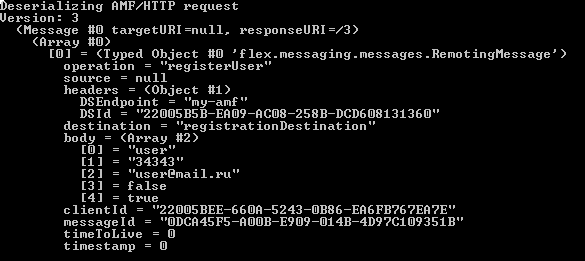
\includegraphics[height=60mm, width=120mm]{fig/development/deserialisedMessage.png}}
\caption{Десериализованное сообщение}
\label{ris:deserialisedMessage.png}
\end{figure} 

\subsection{AMF клиент}

В BlazeDS существует механизм, Java AMF Client, позволяющий совершать удалённые вызовы методов и обрабатывать ответы
сервера. Преимущество использования Java AMF Client заключается в том, что сериализация и десериализация AMF сообщений,
отправляемых клиентом и сервером, а также установка http соединения, полностью обеспечивается данной технологией.

Классы, реализующие функционал Java AMF Client, находятся в пакете flex.messaging.io.amf.client. Основным классом
является AMFConnection. Пример его работы показан ниже.

ТУТ ПРИМЕР КОДА

AMFConnection устанавливает соединение с удалённым объектом по указанному URL с помощью метода connect().
В случае успешной установки соединения метод call() отправляет AMF запрос пользователю, в качестве параметров метод
принимает имя вызываемого на стороне сервера метода и его параметры, представленные в виде массива объектов.

В данном примере возможно появление двух видов исключительных ситуаций:

\begin{enumerate}
\item ServerStatusException --- в случае появления сообщения об ошибке от сервера.
\item ClientStatusException --- в случае ошибки установки соединения с сервером или при непредвиденном разрыве
соединения.
\end{enumerate}

\section{Интеграция с JMeter}

\subsection{Общая архитектура JMeter}

Структура проекта JMeter изображена на ...

ТУТ РИСУНОК

\begin{enumerate}
\item bin --- содержит в себе .bat и .sh файлы для запуска JMeter, файл ApacheJMeter.jar и файлы настроек;
\item docs --- директория, содержащая документацию по проекту;
\item extras --- дополнительне фалйлы для утилиты ant;
\item lib --- jar файлы библиотек, используемых в JMeter;
\item lib/ext --- jar файлы ядра и отдельных компонентов JMeter;
\item src --- исходные коды JMeter;
\item test --- юнит-тесты;
\item xdocs --- xml файлы для документации (JMeter генерирует документацию из xml).
\end{enumerate}

Рассмотрим подробнее содержимое директории src:

\begin{enumerate}
\item component --- директория, содержащая общие для различных протоколов элементы, такие как визуалайзеры,
соответствия и т.д;
\item core --- ядро JMeter, содержит базовые интерфейсы и абстрактные классы;
\item examples --- примеры, демонстрирующие использование компонентов фреймворка;
\item functions --- стандартные функции, используемые всеми компонентами;
\item jorphan --- утилитные классы;
\item monitor --- элементы мониторинга сервера Tomcat 5;
\item protocol --- содержит реализации компонентов Jmeter для различных протоколов.
\end{enumerate}

В архитектуре JMeter ядро, содержащее в себе интерфейсы и абстрактные классы,а также базовый функционал,
отделёны от конкретных реализаций компонентов для различных протоколов. Это сделано для того, чтобы разработчики
могли добавлять поддержку новых протоколов без сборки всего приложения. Таким образом, для того, чтобы добавить
в JMeter элементы тестирования Flex приложений, нужно будет переопределить несколько базовых
компонентов JMeter, собрать jar файл модуля, и поместить его в директорию lib/ext --- новый функционал будет
автоматически подхвачен JMeter.

Прежде чем приступить к созданию различных компонентов, опишем ряд общих правил их реализации,
которые необходимы для того, чтобы элемент правильно работал в среде JMeter. В основном это относится к
графическому интерфейсу пользователя (GUI).

В JMeter код GUI элемента отделён от функционального кода элемента, поэтому реализуя новый компонент следует
создавать отдельные классы для рабочего функционала и графического представления. GUI элемент, в зависимости
 от его предназанчения, должен расширять один из представленных ниже абстрактных классов.

\begin{enumerate}
\item AbstractSamplerGui
\item AbstractAssertionGui
\item AbstractConfigGui
\item AbstractControllerGui
\item AbstractPostProcessorGui
\item AbstractPreProcessorGui
\item AbstractVisualizer
\item AbstractTimerGui
\end{enumerate}

Следующим шагом является реализация метода getResourceLabel().Этот метод должен возвращать имя ресурса,
представляющего компонент.

Чтобы GUI создаваемого вами тестового элемента соответсвовало стилю JMeter, следует добавить в него стандартную
рамку JMeter, которая создаётся следующим образом --- setBorder(makeBorder()). Также необходимо создать
панель с именем элемента методом makeTitlePanel(). Обычно её располагают в верхней центральной части панели
элемента.

Важным пунктом является реализация метода public void configure(TestElement el), который отвечает за отображение
параметров тестового элемента в GUI. Первой строчкой в методе должен быть вызов super.configure(e), что обеспечит
выполнение некоторых стандартных действий, как например отображение имени элемента. Обратное действие ---
передача данных из GUI в тестовый элемент --- обеспечивается методом public void modifyTestElement(TestElement e),
который также нужно реализовать. В имплиментацию этого метода тоже включается строчка
super.configureTestElement(e).

Другой необходимый в создании GUI метод --- public TestElement createTestElement(). Он должен новый экземпляр
тестового элемента и передавать его в метод modifyTestElement(TestElement) в качестве параметра.

Все вышеобозначенные правила разграничения GUI и функционала элемента облегчают разработчикам реализацию графического
интерфейса. Хотя программист и не освобождается от процедуры создания и размещения компонентов графического
интерфейса, всё взаимодействие GUI и соответствующего ему тестового элемента обеспечивается JMeter.

\subsection{Реализация модуля отправки AMF сообщений}

Согласно одному из требований технического задания, разрабатываемое программное обеспечение должно предоставлять возможность 
отправки AMF сообщения серверу. Данное требование осуществляется реализацией такого компонента JMeter, как сэмплер(Sampler). 
Сэмлеры в JMeter предназначены для отправки запросов серверу и ожидания ответов от них. 

Чтобы добавить свой собственный сэмплер в JMeter, необходимо создать класс, наследующий абстрактный класс AbstractSampler и 
реализующий метод public SampleResult sample(Entry e). Именно этот метод будет вызываться у каждого сэмплера, входящего в 
тест план во время его прогона. Метод sample должен осуществлять подключение к серверу, ожидание ответа от него и возвращать 
экземпляр класса SampleResult, содержащий в себе информацию о выполнении запроса.

В рамках решения этой задачи был создан класс AmfRPCSampler. В методе sample данного класса производится вызов метода 
удалённого объекта на стороне сервера с помощью AMF клиента (алгоритм работы AMF клиента описан в разделе 3.2.3). 
Метод возвращает экземпляр класса AmfRPCSamplerResult, в который по ходу выполнения метода sample записывается информация 
о передаваемых в запросе данных, ответ сервера, а также статус выполнения запроса (в случае, если отсет сервера получен и 
не содержит сообщений обошибках, запрос считается успешно выполненным).

Также метод sample класса AmfRPCSampler отвечает за одно из важных технических требований к модулю --- возможность проведения 
полноценных нагрузочных тестов. В JMeter имитация работы с приложением большого числа пользователей одновременно осуществляется 
засчёт запуска тест-плана в несколько потоков и реализуемый сэмплер должен обеспечивать уникальность идентификатора сессии AMF 
клиента с сервером для каждого потока, выполняющего тест-план, а также гарантировать его сохранность в рамках одного потока. 
Данная задача решается засчёт введения в классе AmfRPCSampler статической переменной ThreadLocal<AMFConnection> AMF_CONNECTION_THREAD_LOCAL. 
Работа с данной переменной происходит следующим образом. В методе sample проверяется текущее значение AMF_CONNECTION_THREAD_LOCAL 
вызовом метода AMF_CONNECTION_THREAD_LOCAL.get(), который возвращает экземпяр AMFConnection для текущего потока. 
Если соединение AMFConnection для данного потока уже было создано, то дальнейшая работа осуществляется с полученным экземпляром 
AMFConnection. Если вызов AMF_CONNECTION_THREAD_LOCAL.get() возвращает null, то создаётся новый экземпляр AMFConnection, производится попытка 
подключения к серверу и значение AMFConnection записывается в AMF_CONNECTION_THREAD_LOCAL. Таким образом все элементы AmfRPCSampler, 
запускаемые одним потоком, будут работать с одним и тем же экземпляром AMFConnection, а остальные потоки будут использовать другие 
соединения.

Разработанный AmfRPCSampler также имеет графический интерфейс пользователя, реализованный в классе AmfRPCSamplerGui. AmfRPCSamplerGui 
создан согласно правилам реализации GUI в JMeter и расширяет класс AbstractSamplerGui. Интерфейс содержит следующие компоненты для ввода данных, 
необходимых для вызова метода объекта на стороне сервера:

\begin{enumerate}
\item endpointUrlField --- поле для URL, по которому отправляется запрос;
\item amfCallField --- поле для имени процедуы, которая должна быть вызвана; 
\item parametersPanel --- таблица параметров вызываемого метода.
\end{enumerate}    

\subsection{Реализация прокси-сервера}

Создание прокси-сервера необходимо для возможности записи трафика между приложением и сервером и дальнейшего использования 
записанных запросов в тест-плане. В рамках модуля реализован прокси сервер, который запускается по адресу 
localhost:port (порт указывается ползователем), обрабатывает полученные http запросы и отправляет их адресату. 
В случае, если тело полученного http запроса содержит AMF сообщение, происходит его десериализация с использованием 
AmfMessageDeserializer и создаётся экземпляр 
AmfRPCSampler, в который записывается информация из AMF сообщения. Все созданные во время работы прокси-сервера AMF запросы 
могут быть перенесены в тест план.

GUI прокси-сервера содержит поле для ввода порта, на котором сервер будет запущен, а также кнопки для запуска и остановки 
сервера.

\section{Тестирование}

Тестирование программного обеспечения --- проверка соответствия между реальным и ожидаемым поведением программы,
осуществляемая на конечном наборе тестов, выбранном определенным образом.
[IEEE Guide to Software Engineering Body of Knowledge, SWEBOK, 2004] В более широком смысле, тестирование - это
одна из техник контроля качества, включающая в себя активности по планированию работ (Test Management),
проектированию тестов, выполнению тестирования и анализу полученных результатов.
Тестирование является важным и неотъемлемым этапом жизненного цикла программного обеспечения, оно позволяет выявить
ошибки уже на ранних стадиях разработки, что сокращает время разработки
и повышает надежность программного продукта. При разработке модуля использовались следующие виды тестирования:

\begin{enumerate}
\item Компонентное (модульное) тестирование(Unit Testing);
\item Приёмочное тестирование.
\end{enumerate}

\subsection{Модульное тестирование}

Компонентное (модульное) тестирование(Unit Testing) проверяет функциональность и ищет дефекты в частях
приложения, которые доступны и могут быть протестированы по-отдельности (модули программ, объекты, классы, функции
и т.д.). Идея состоит в том, чтобы писать тесты для каждой нетривиальной функции или метода. Это позволяет достаточно
быстро проверить, не привело ли очередное изменение кода к регрессии, то есть к появлению ошибок в уже оттестированных
местах программы, а также облегчает обнаружение и устранение таких ошибок. Цель модульного тестирования --- изолировать
отдельные части программы и показать, что по отдельности эти части работоспособны. Этот тип тестирования обычно
выполняется программистами.

Во процессе реализации модуля было осуществлено покрытие классов, заключающих в себе основной функционал, юнит-тестами
(классы, реализующие GUI, тестами не покрывались). Тестирование проводилось с помощью JUnit ---  библиотеки для
модульного тестирования программного обеспечения на языке Java. Использование Maven в разработке приложения гарантирует,
что все созданные юнит-тесты будут автоматически запускаться перед сборкой модуля, и в случае, если хотя бы один тест не
выполнится, сборка приложения не будет запущена.

Как и любая технология тестирования, модульное тестирование не позволяет отловить все ошибки программы. В самом деле,
это следует из практической невозможности трассировки всех возможных путей выполнения программы, за исключением
простейших случаев. Кроме того, происходит тестирование каждого из модулей по отдельности. Это означает, что ошибки
интеграции, системного уровня, функций, исполняемых в нескольких модулях не будут определены. Кроме того, данная
технология бесполезна для проведения тестов на производительность. Таким образом, модульное тестирование более
эффективно при использовании в сочетании с другими методиками тестирования.

\subsection{Приёмочное тестирование}

Приемочное тестирование или Приемо-сдаточное испытание (Acceptance Testing) представляет собой формальный процесс
тестирования, который проверяет соответствие системы требованиям и проводится с целью:

\begin{enumerate}
\item определения удовлетворяет ли система приемочным критериям;
\item вынесения решения заказчиком или другим уполномоченным лицом принимается приложение или нет.
\end{enumerate}

Приемочное тестирование выполняется на основании набора типичных тестовых случаев и сценариев, разработанных на
основании требований к данному приложению.Решение о проведении приемочного тестирования принимается, когда:

\begin{enumerate}
\item продукт достиг необходимого уровня качества;
\item заказчик ознакомлен с Планом Приемочных Работ (Product Acceptance Plan);
\end{enumerate}

Фаза приемочного тестирования длится до тех пор, пока заказчик не выносит решение об отправлении приложения на
доработку или выдаче приложения.

План Приемочных Испытаний -  это документ, описывающий весь объем работ по тестированию, начиная с описания объекта,
стратегии, расписания, критериев начала и окончания тестирования, до необходимого в процессе работы оборудования,
специальных знаний, а также оценки рисков с вариантами их разрешения.

Также важным этапом в подготовке приёмочного тестирования является проектирование тестовых случаев (Test Cases) ---
артефактов, описывающих совокупность шагов, конкретных условий и параметров, необходимых для проверки реализации
тестируемой функции или её части. Чаще всего test case состоит из трёх частей:

\begin{enumerate}
\item предусловия --- список действий, которые приводят систему к состоянию пригодному для проведения основной
проверки, либо список условий, выполнение которых говорит о том, что система находится в пригодном для проведения
основного теста состоянии;
\item шаги теста --- список действий, переводящих систему из одного состояния в другое, для получения
результата, на основании которого можно сделать вывод о удовлетворении реализации, поставленным требованиям;
\item Expected Results --- описание состояния системы, в котором она должна находиться после выполнения шагов теста.
\end{enumerate}

Набор тестов должен быть спроектирован таким образом, чтобы обеспечивать оптимальное тестовое покрытие тестируемого
приложения.

План приёмочных испытаний, а также набор тест кейзов, используемых при тестировании разработанного модуля находятся в приложении к 
к диплому.

